% Standalone draft of the SEAL positioning figure.
% Build:  pdflatex positioning_figure.tex   (produces positioning_figure.pdf)
% Story:  the task automaton (a->b->c->d) is SHARED by TLI, GLiDE, and SEAL.
%         The three methods differ ONLY in how the localization function L
%         (continuous state -> current mode) is obtained.
\documentclass[border=8pt]{standalone}
\usepackage{tikz}
\usepackage{amsmath}
\usetikzlibrary{positioning,arrows.meta,shapes.geometric,fit,backgrounds}

\definecolor{seal}{RGB}{0,140,90}
\definecolor{glide}{RGB}{200,120,0}
\definecolor{tli}{RGB}{80,80,80}

\begin{document}
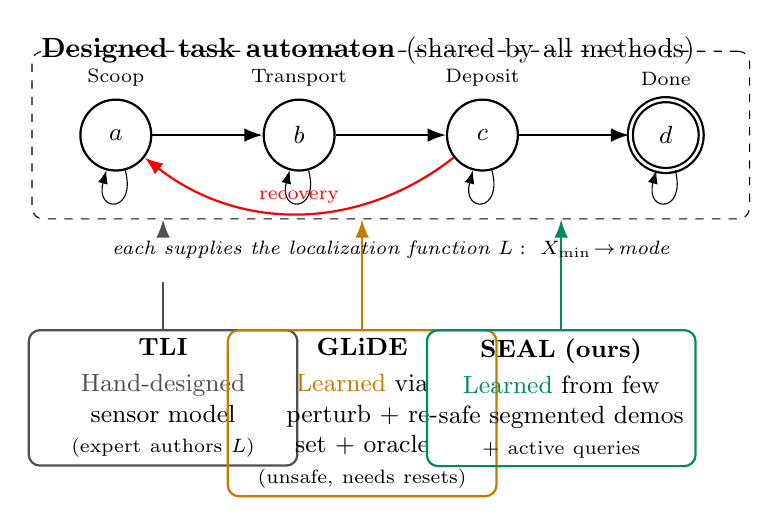
\begin{tikzpicture}[
  >=Latex, font=\small,
  mode/.style={circle, draw, thick, minimum size=9mm, inner sep=0pt},
  Lbox/.style={rounded corners, draw, thick, align=center, text width=32mm,
               minimum height=15mm, inner sep=3pt},
  lbl/.style={font=\scriptsize\itshape},
]

% ---------- Shared automaton (top) ----------
\node[mode] (a) {$a$};
\node[mode, right=14mm of a] (b) {$b$};
\node[mode, right=14mm of b] (c) {$c$};
\node[mode, right=14mm of c, double, double distance=1pt] (d) {$d$};

\node[above=1pt of a, font=\scriptsize] {Scoop};
\node[above=1pt of b, font=\scriptsize] {Transport};
\node[above=1pt of c, font=\scriptsize] {Deposit};
\node[above=1pt of d, font=\scriptsize] {Done};

\draw[->,thick] (a) -- (b);
\draw[->,thick] (b) -- (c);
\draw[->,thick] (c) -- (d);
% self-loops (dwell in mode)
\foreach \n in {a,b,c,d}{\draw[->] (\n) edge[loop below, looseness=6, min distance=4mm] (\n);}
% recovery edge (perturbation re-localizes to an earlier mode)
\draw[->, thick, red] (c) to[bend left=38] node[above, font=\scriptsize, red] {recovery} (a);

% frame + title for the shared automaton
\begin{scope}[on background layer]
  \node[draw, dashed, rounded corners, inner sep=6mm, fit=(a)(b)(c)(d)] (auto) {};
\end{scope}
\node[anchor=west, font=\bfseries] at (auto.north west) {Designed task automaton \normalfont(shared by all methods)};

% ---------- Three localization boxes (bottom) ----------
\node[Lbox, draw=tli,   text=black, below=20mm of a.south, xshift=6mm]  (tli)   {\textbf{TLI}\\[2pt] \textcolor{tli}{Hand-designed}\\ sensor model\\ \scriptsize(expert authors $L$)};
\node[Lbox, draw=glide, below=20mm of b.south, xshift=8mm] (glide) {\textbf{GLiDE}\\[2pt] \textcolor{glide}{Learned} via\\ perturb + reset + oracle\\ \scriptsize(unsafe, needs resets)};
\node[Lbox, draw=seal,  below=20mm of c.south, xshift=10mm] (seal)  {\textbf{SEAL (ours)}\\[2pt] \textcolor{seal}{Learned} from few\\ safe segmented demos\\ \scriptsize+ active queries};

% arrows: each method grounds/localizes onto the SAME automaton
\draw[->, thick, tli]   (tli.north)   -- ++(0,6mm) node[lbl, tli, above right, xshift=-4mm] {} (auto.south -| tli.north);
\draw[->, thick, glide] (glide.north) -- (auto.south -| glide.north);
\draw[->, thick, seal]  (seal.north)  -- (auto.south -| seal.north);

\node[lbl, below=1.5mm of auto.south] {each supplies the localization function $L:\ X_{\min}\!\to\!\text{mode}$};

\end{tikzpicture}
\end{document}
